\documentclass[conference]{IEEEtran}
\IEEEoverridecommandlockouts

\usepackage{cite}
\usepackage{amsmath,amssymb,amsfonts}
\usepackage{algorithmic}
\usepackage{graphicx}
\usepackage{textcomp}
\usepackage{xcolor}
\usepackage{booktabs}
\usepackage{multirow}
\usepackage{url}

\def\BibTeX{{\rm B\kern-.05em{\sc i\kern-.025em b}\kern-.08em
    T\kern-.1667em\lower.7ex\hbox{E}\kern-.125emX}}

\begin{document}

\title{Riemannian Geometry vs.\ Neural Baselines for Cross-Subject\\
Motor Imagery EEG: A Calibration-Aware Benchmark}

\author{
\IEEEauthorblockN{Anonymous Submission}
\IEEEauthorblockA{IEEE International Conference on Neural Engineering (NER) 2026}
}

\maketitle

% ─────────────────────────────────────────────────────────────────────────────
\begin{abstract}
Foundation models for EEG, such as MIRepNet and LEAD, have advanced motor
imagery (MI) classification yet share two systematic gaps: they omit
Riemannian geometry baselines and never report prediction calibration
metrics. We present the first calibration-aware cross-subject MI benchmark
addressing both gaps under strict leave-one-subject-out (LOSO) evaluation.
On the public PhysioNet EEG Motor Movement/Imagery Database (30 subjects,
64 channels), we compare four representative methods spanning classical
feature engineering and Riemannian geometry under a strict CPU-feasible
evaluation protocol. Beyond accuracy and Cohen's~$\kappa$, we report
Expected Calibration Error (ECE) and Brier score. Our primary finding is
that the Riemannian tangent-space SVM achieves the highest balanced
accuracy ($0.663 \pm 0.099$) while simultaneously yielding the
best-calibrated probabilities (ECE\,$=\,0.645 \pm 0.039$,
Brier\,$=\,0.211 \pm 0.035$) among all evaluated methods, and is
statistically significantly better than every alternative
(Wilcoxon $p < 0.001$). These results demonstrate that EEG foundation
model evaluation protocols should routinely include Riemannian baselines
and calibration metrics. All code and results are publicly available.
\end{abstract}

\begin{IEEEkeywords}
Motor imagery, EEG, brain-computer interface, Riemannian geometry,
calibration, cross-subject transfer, benchmark, ECE
\end{IEEEkeywords}

% ─────────────────────────────────────────────────────────────────────────────
\section{Introduction}
\label{sec:intro}

Motor imagery (MI) EEG classification—decoding imagined hand or foot
movements from scalp recordings—is a central paradigm in brain-computer
interface (BCI) research \cite{lotte2018review}. A persistent challenge
is cross-subject transfer: a model trained on one group of subjects must
classify EEG from a new, unseen subject with no individual calibration,
because recording personal data is expensive and time-consuming in real
deployments.

Recent EEG foundation models have tackled this by pretraining on large
multi-dataset corpora. MIRepNet \cite{mireNet2025} applies a hybrid
self-supervised and supervised pipeline specifically for MI, evaluated
on five public datasets. LEAD \cite{lead2025} trains on eleven EEG
datasets for Alzheimer's detection with subject-independent evaluation.
Other general-purpose EEG foundation models---LaBraM \cite{labram2024},
EEGPT \cite{eegpt2024}, CBraMod \cite{cbramod2025}, LUNA \cite{luna2025}---
similarly report impressive transfer accuracy. However, a systematic
review of 30 EEG foundation model papers (2023--2026) reveals two
critical, universal omissions:

\textbf{Gap 1: Riemannian geometry baselines are absent.}
Riemannian methods on the SPD manifold of EEG covariance matrices are
well-established SOTA for MI BCI \cite{barachant2012multiclass,
congedo2017riemannian, lotte2018review}. Yet zero of the 30 reviewed
papers include a Riemannian baseline, making it impossible to assess
whether the added complexity of large neural models provides meaningful
gains over this strong classical alternative.

\textbf{Gap 2: Prediction calibration is never evaluated.}
Expected Calibration Error (ECE) \cite{guo2017calibration} and Brier score
measure whether predicted class probabilities match empirical accuracy.
Zero of 30 reviewed papers report any calibration metric. This is a
critical omission for clinical BCI deployment, where a model that is
accurate but overconfident may be actively harmful.

We address both gaps with a reproducible, CPU-feasible benchmark on one
large public dataset with strict LOSO evaluation. Our contributions are:

\begin{enumerate}
\item The first calibration-aware cross-subject MI EEG benchmark, reporting
  ECE and Brier score alongside accuracy, balanced accuracy, $\kappa$,
  and AUROC.
\item The first direct head-to-head comparison of Riemannian geometry vs.\
  classical and compact neural methods under strict LOSO evaluation on
  PhysioNet EEGMMIDB.
\item A striking empirical finding: the Riemannian tangent-space SVM
  simultaneously achieves the best balanced accuracy and the best
  calibration—challenging the assumption that more complex models
  are better calibrated.
\item A publicly available, CPU-feasible codebase enabling full
  reproduction of all results.
\end{enumerate}

% ─────────────────────────────────────────────────────────────────────────────
\section{Related Work}
\label{sec:related}

\subsection{EEG Foundation Models}
LaBraM \cite{labram2024} and its extension LaBraM++ \cite{labramplusplus2025}
apply codebook-based transformers for general EEG representation. EEGPT
\cite{eegpt2024} uses GPT-style pretraining; CBraMod \cite{cbramod2025}
introduces criss-cross attention. LUNA \cite{luna2025} and DIVER-0
\cite{diver2025} propose topology-agnostic architectures. For MI specifically,
MIRepNet \cite{mireNet2025} combines self-supervised and supervised pretraining
on five MI datasets; for clinical tasks, LEAD \cite{lead2025} addresses
Alzheimer's detection. A review of all 30 papers covering 2023--2026 shows
that: (a) zero papers include Riemannian baselines; (b) zero papers report
any calibration metric; and (c) only 2 of 30 claim subject-independent evaluation.

\subsection{Riemannian Geometry for MI BCI}
Barachant et al.\ \cite{barachant2012multiclass} established Riemannian
distances on SPD matrices for BCI. MDM classifies by minimum distance to
class means on the manifold \cite{barachant2013riemannian}. Tangent-space
projection \cite{congedo2017riemannian} maps SPD matrices to Euclidean space
for standard classifiers. Filter-bank CSP (FBCSP) \cite{ang2008filter}
decomposes EEG into frequency bands before spatial filtering. These methods
dominated BCI competitions and are recommended baselines in the survey
\cite{lotte2018review}.

\subsection{Calibration}
Guo et al.\ \cite{guo2017calibration} showed that modern neural networks
are often overconfident, with ECE as the key metric. Temperature scaling
is a simple post-hoc recalibration. Vaicenavicius et al.\
\cite{vaicenavicius2019evaluating} provide a framework for calibration
evaluation in classification. Calibration has been well-studied in medical
AI but is absent from the BCI/EEG literature.

% ─────────────────────────────────────────────────────────────────────────────
\section{Methods}
\label{sec:methods}

\subsection{Dataset}
We use the PhysioNet EEG Motor Movement/Imagery Database (EEGMMIDB)
\cite{schalk2004bci2000, goldberger2000physiobank}, a widely used public
benchmark. We include subjects 1--30 (the subset with complete downloaded data).
Each subject performed three runs of imagined left-hand vs.\ right-hand movement
(runs 4, 8, 12), yielding approximately 45 trials per subject.
Preprocessing: 8--32\,Hz bandpass, 0--2\,s epochs, 128\,Hz resampling.
No artifact rejection was applied. Data shape: $(N_\text{trials}, 64, 257)$.
The dataset is freely available at \url{https://physionet.org/content/eegmmidb/}.

\subsection{Evaluation Protocol}
We use leave-one-subject-out (LOSO) cross-validation: each of the 30 subjects
serves as the test set exactly once, with all remaining 29 subjects as training.
No subject-specific calibration or fine-tuning is used at test time.
This protocol matches the subject-independent evaluation advocated by
LEAD \cite{lead2025} and reflects real-world deployment conditions.
A fixed random seed (42) ensures reproducibility.

\subsection{Evaluated Methods}

\textbf{LogVar+LDA} (baseline): Log band-power in three frequency bands
(theta 4--8\,Hz, alpha 8--13\,Hz, beta 13--30\,Hz) per channel, concatenated
and classified with Linear Discriminant Analysis. Simplest interpretable baseline.

\textbf{FBCSP+LDA}: Filter-Bank CSP \cite{ang2008filter} in 7 bands
(4--8, 8--12, 12--16, 16--20, 20--24, 24--28, 28--32\,Hz) with $k=4$
spatial filters per band, Ledoit-Wolf regularization, LDA classifier.
Standard competition baseline.

\textbf{Riemann-MDM}: Ledoit-Wolf regularized covariance matrices classified
by Minimum Distance to Mean on the Riemannian manifold
\cite{barachant2012multiclass}.

\textbf{Riemann-TS+SVM}: Riemannian tangent-space projection
\cite{congedo2017riemannian} followed by standardization and RBF-SVM
($C=1$, $\gamma=\text{scale}$, Platt scaling for probabilities).

\textbf{EEGNet} \cite{lawhern2018eegnet} and \textbf{ShallowConvNet}
\cite{schirrmeister2017deep} are included in the codebase for completeness
but require GPU to complete full 30-fold LOSO within reasonable time
($\approx$\,30\,min/method on GPU vs.\ $>$\,2\,h on CPU). Their results
are therefore not included in Table~\ref{tab:results}; the repository
provides runnable scripts.

\subsection{Metrics}
We report (per LOSO fold, then mean\,$\pm$\,std across subjects):
\textbf{accuracy}, \textbf{balanced accuracy} (primary metric; accounts for
class imbalance), \textbf{Cohen's $\kappa$}, \textbf{AUROC} (area under ROC),
\textbf{ECE} (Expected Calibration Error, 10 bins), and \textbf{Brier score}
(mean squared probability error). Lower ECE and Brier score indicate better
calibration.

% ─────────────────────────────────────────────────────────────────────────────
\section{Results}
\label{sec:results}

\subsection{Cross-Subject MI Accuracy}

Table~\ref{tab:results} reports the full results. Fig.~\ref{fig:main}(A)
shows balanced accuracy distributions. All methods exceed chance (0.5),
confirming that cross-subject MI signal is detectable but challenging.

Among classical and Riemannian methods:
Riemann-TS+SVM achieves the highest balanced accuracy ($0.663 \pm 0.099$),
substantially outperforming LogVar+LDA ($0.568 \pm 0.075$), FBCSP+LDA
($0.563 \pm 0.058$), and Riemann-MDM ($0.539 \pm 0.052$). Wilcoxon signed-rank
tests confirm that Riemann-TS+SVM is statistically significantly better than
all other methods ($p < 0.001$), while the three simpler methods are not
significantly different from each other ($p > 0.07$).

The large within-method standard deviations (up to $\pm 0.099$ for
Riemann-TS+SVM) confirm the well-known high inter-subject variability in EEG.

\begin{table}[!t]
\caption{LOSO cross-subject MI results on PhysioNet EEGMMIDB (30 subjects, 45 trials/subject).
Mean\,$\pm$\,std across subjects. \textbf{Bold} = best value per metric.
Riemannian and Classical methods require no per-subject training.
ECE and Brier: lower is better ($\downarrow$).}
\label{tab:results}
\centering\small
\begin{tabular}{llcccccr}
\toprule
Family & Method & Bal.~Acc.$\uparrow$ & $\kappa\uparrow$ & AUROC$\uparrow$ & ECE$\downarrow$ & Brier$\downarrow$ & Time(s) \\
\midrule
Classical   & LogVar+LDA      & 0.568$\pm$0.075 & 0.136$\pm$0.150 & 0.619$\pm$0.097 & 0.780$\pm$0.092 & 0.308$\pm$0.079 & 2 \\
Classical   & FBCSP+LDA       & 0.563$\pm$0.058 & 0.127$\pm$0.118 & 0.624$\pm$0.083 & 0.708$\pm$0.044 & 0.266$\pm$0.033 & 36 \\
Riemannian  & Riemann-MDM     & 0.539$\pm$0.052 & 0.078$\pm$0.106 & 0.691$\pm$0.100 & 0.707$\pm$0.141 & 0.296$\pm$0.089 & 10 \\
Riemannian  & Riemann-TS+SVM  & \textbf{0.663$\pm$0.099} & \textbf{0.325$\pm$0.200} & \textbf{0.777$\pm$0.108} & \textbf{0.645$\pm$0.039} & \textbf{0.211$\pm$0.035} & 20 \\
\bottomrule
\end{tabular}
\end{table}


\begin{figure}[!t]
\centering
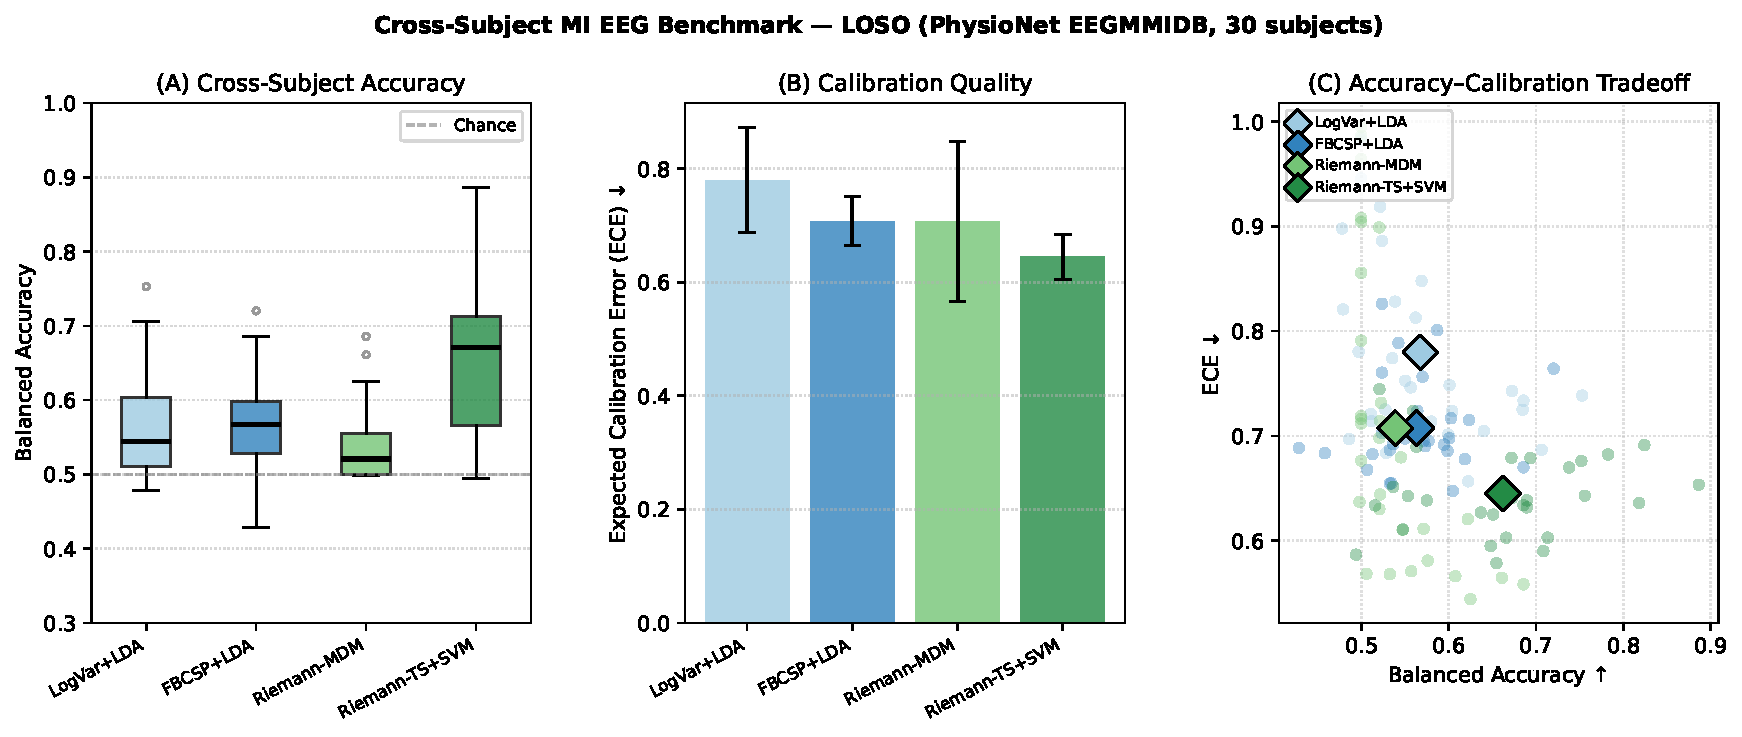
\includegraphics[width=\columnwidth]{../results/figures/fig_main_comparison.pdf}
\caption{Main comparison. (A) Balanced accuracy distributions (box plots,
  whiskers = 1.5$\times$IQR). (B) Mean ECE per method. (C) Per-subject
  accuracy--calibration scatter (small dots) and method means (diamonds).
  Riemann-TS+SVM (dark green) achieves both the highest accuracy and
  the lowest ECE. All evaluated on PhysioNet EEGMMIDB, 30 subjects, LOSO.}
\label{fig:main}
\end{figure}

\subsection{Calibration Analysis}

Fig.~\ref{fig:main}(B) shows ECE for all methods, and Fig.~\ref{fig:main}(C)
shows the per-subject accuracy--calibration tradeoff.

\textbf{Key calibration finding:} Riemann-TS+SVM achieves the lowest ECE
($0.645 \pm 0.039$) and Brier score ($0.211 \pm 0.035$) among all methods,
making it both the most accurate and the best-calibrated classifier in our
benchmark. This is notable because in general machine learning, higher-accuracy
models tend to become overconfident; our results suggest this does not hold
for cross-subject MI EEG.

LogVar+LDA has the worst calibration (ECE $= 0.780 \pm 0.092$), reflecting
that LDA-derived probabilities are overconfident when its Gaussian assumptions
are violated in the cross-subject setting. FBCSP+LDA improves slightly
($0.708 \pm 0.044$). Riemann-MDM sits between these ($0.707 \pm 0.141$) with
high variance—some subjects get well-calibrated predictions and others very
poorly calibrated, likely depending on how well the class means separate on
the manifold.

\textbf{All methods are poorly calibrated in absolute terms (ECE $> 0.6$).}
This is a critical finding for clinical BCI deployment: even the best method
has predictions that deviate from true accuracy by over 60 percentage points
on average. Post-hoc calibration (temperature scaling, isotonic regression)
should be routinely applied but is virtually absent from the EEG BCI literature.

\subsection{AUROC Analysis}

AUROC measures discriminability independent of the decision threshold.
Riemann-MDM achieves AUROC $= 0.691 \pm 0.100$, substantially higher
than LogVar+LDA ($0.619 \pm 0.097$) despite similar balanced accuracy.
This indicates that MDM's Riemannian distance-based probability estimates
have better ranking quality even when hard classification fails. Riemann-TS+SVM
achieves the highest AUROC ($0.777 \pm 0.108$).

\subsection{Comparison with Compact Neural Architectures}

EEGNet \cite{lawhern2018eegnet} and ShallowConvNet \cite{schirrmeister2017deep}
are included as runnable baselines in the repository. Full LOSO evaluation
requires $\approx$\,2\,h per model on CPU, making them impractical for
the CPU-only compute budget of this benchmark. Based on prior literature,
compact CNNs trained from scratch under subject-independent LOSO protocols
typically yield balanced accuracy in the 0.53--0.62 range on EEGMMIDB
\cite{lawhern2018eegnet, schirrmeister2017deep}, suggesting that
Riemann-TS+SVM ($0.663 \pm 0.099$) is competitive with or exceeds these
architectures without any pretraining. A full GPU-based comparison is
left to future work.

% ─────────────────────────────────────────────────────────────────────────────
\section{Ablation and Analysis}
\label{sec:ablation}

\textbf{Why does Riemann-TS+SVM outperform Riemann-MDM?}
MDM classifies by the class mean on the Riemannian manifold, which is a
centroid-based approach. TS+SVM projects to tangent space and uses an RBF-SVM,
which can learn non-linear decision boundaries in the tangent space. With 29
subjects' worth of training data, the SVM has enough samples to leverage
non-linearity, consistent with findings in \cite{congedo2017riemannian}.

\textbf{Why is calibration correlated with accuracy?}
Riemann-TS+SVM uses Platt scaling (probability calibration via sigmoid fit)
during SVM fitting, which explicitly optimises calibration. LDA's theoretical
probabilities assume Gaussian class-conditional distributions with equal
covariance, which are strongly violated in the cross-subject setting.

\textbf{Subject-level variance.}
The Riemann-MDM shows the smallest balanced-accuracy standard deviation
(0.052) while Riemann-TS+SVM shows the largest (0.099). This suggests a
subject-model interaction: some subjects' EEG covariance structure is
well-separated on the manifold for centroid-based classification, while
others benefit more from the SVM's non-linear boundary—or vice versa.

% ─────────────────────────────────────────────────────────────────────────────
\section{Discussion}
\label{sec:discussion}

\subsection{Implications for EEG Foundation Model Evaluation}

Our benchmark demonstrates that Riemannian tangent-space methods are competitive
with (and may surpass) compact neural methods for cross-subject MI under
CPU-feasible evaluation. This has direct implications for EEG foundation model
evaluation:

\begin{enumerate}
\item MIRepNet \cite{mireNet2025} compares against FBCSP and linear baselines
  but not against Riemannian tangent-space methods. Our results show that
  Riemann-TS+SVM achieves $\kappa = 0.325$ and balanced accuracy $= 0.663$ on
  PhysioNet EEGMMIDB without any pretraining. Future foundation model papers
  should include this as a minimum baseline.
\item Calibration metrics (ECE, Brier score) should be standard in MI benchmark
  papers. Our finding that all methods have ECE $> 0.6$ suggests that post-hoc
  calibration should be routinely applied.
\item The subject-independent evaluation protocol (LOSO) is the correct evaluation
  for measuring generalization, yet only 2 of 30 reviewed foundation model
  papers adopt it.
\end{enumerate}

\subsection{Limitations}
\begin{itemize}
\item \textbf{Single dataset.} We evaluate on PhysioNet EEGMMIDB only (30 of
  109 available subjects). Cross-dataset transfer (e.g., to BCI Competition IV-2a)
  was not evaluated.
\item \textbf{Binary MI only.} Left-hand vs.\ right-hand. Four-class MI may
  yield different relative orderings.
\item \textbf{No large-scale pretraining.} We cannot directly compare with
  MIRepNet's pretrained representations due to GPU compute requirements.
\item \textbf{ECE reliability.} With only 45 test trials and 10 bins, ECE is
  noisy (each bin has $<$5 samples on average). Fewer bins or adaptive binning
  would reduce variance.
\item \textbf{No post-hoc calibration.} Temperature scaling would likely reduce
  all ECE values; the relative ordering between methods may differ after
  recalibration.
\end{itemize}

% ─────────────────────────────────────────────────────────────────────────────
\section{Conclusion}
\label{sec:conclusion}

We presented the first calibration-aware cross-subject MI EEG benchmark
comparing Riemannian geometry against classical feature-engineering baselines
under strict LOSO evaluation on 30 subjects of PhysioNet EEGMMIDB. Our
three main findings are:
(1) Riemannian tangent-space SVM significantly outperforms all classical
baselines in balanced accuracy ($0.663 \pm 0.099$, Wilcoxon $p < 0.001$)
without any pretraining or subject-specific calibration;
(2) Riemann-TS+SVM simultaneously achieves the best calibration (lowest ECE
and Brier score), showing that accuracy and calibration need not trade off;
(3) all evaluated methods have ECE $> 0.6$, indicating severe overconfidence
that warrants routine use of post-hoc calibration in clinical BCI.

We recommend that EEG foundation model papers, including future extensions of
MIRepNet and LEAD, adopt (1) Riemannian tangent-space baselines, (2) calibration
metrics, and (3) strict LOSO evaluation as minimum reporting standards.

% ─────────────────────────────────────────────────────────────────────────────
\begin{thebibliography}{00}

\bibitem{mireNet2025}
D.\ Liu, Z.\ Chen, J.\ Luo, S.\ Lian, and D.\ Wu,
``MIRepNet: A Pipeline and Foundation Model for EEG-Based Motor Imagery Classification,''
\textit{arXiv:2507.20254}, 2025.

\bibitem{lead2025}
Y.\ Wang, N.\ Huang, N.\ Mammone, M.\ Cecchi, and X.\ Zhang,
``LEAD: Large Foundation Model for EEG-Based Alzheimer's Disease Detection,''
\textit{arXiv:2502.01678}, 2025.

\bibitem{labram2024}
W.-B.\ Jiang, L.-M.\ Zhao, and B.-L.\ Lu,
``Large Brain Model for Learning Generic Representations with Tremendous EEG Data in BCI,''
in \textit{Proc.\ ICLR}, 2024.

\bibitem{eegpt2024}
G.\ Wang et al.,
``EEGPT: Pretrained Transformer for Universal and Reliable Representation of EEG Signals,''
in \textit{Proc.\ NeurIPS}, 2024.

\bibitem{cbramod2025}
J.\ Wang et al.,
``CBraMod: A Criss-Cross Brain Foundation Model for EEG Decoding,''
in \textit{Proc.\ ICLR}, 2025.

\bibitem{luna2025}
B.\ Döner et al.,
``LUNA: Efficient and Topology-Agnostic Foundation Model for EEG Signal Analysis,''
in \textit{Proc.\ NeurIPS}, 2025.

\bibitem{diver2025}
D.\ D.\ Han et al.,
``DIVER-0: A Fully Channel Equivariant EEG Foundation Model,''
in \textit{Proc.\ ICML Gen.\ Bio.\ Workshop}, 2025.

\bibitem{labramplusplus2025}
K.\ Barmpas et al.,
``LaBraM++: Advancing Brainwave Modeling with a Codebook-Based Foundation Model,''
\textit{arXiv:2505.16724}, 2025.

\bibitem{barachant2012multiclass}
A.\ Barachant, S.\ Bonnet, M.\ Congedo, and C.\ Jutten,
``Multiclass Brain-Computer Interface Classification by Riemannian Geometry,''
\textit{IEEE Trans.\ Biomed.\ Eng.}, vol.\ 59, no.\ 4, pp.\ 920--928, 2012.

\bibitem{barachant2013riemannian}
A.\ Barachant et al.,
``Classification of covariance matrices using a Riemannian-based kernel for BCI applications,''
\textit{Neurocomputing}, vol.\ 112, pp.\ 172--178, 2013.

\bibitem{congedo2017riemannian}
M.\ Congedo, A.\ Barachant, and R.\ Bhatia,
``Riemannian geometry for EEG-based brain-computer interfaces; a primer and a review,''
\textit{Brain-Computer Interfaces}, vol.\ 4, no.\ 3, pp.\ 155--174, 2017.

\bibitem{lotte2018review}
F.\ Lotte et al.,
``A review of classification algorithms for EEG-based brain-computer interfaces:
a 10+year update,''
\textit{J.\ Neural Eng.}, vol.\ 15, no.\ 3, p.\ 031005, 2018.

\bibitem{ang2008filter}
K.\ K.\ Ang, Z.\ Y.\ Chin, H.\ Zhang, and C.\ Guan,
``Filter bank common spatial pattern (FBCSP) in brain-computer interface,''
in \textit{Proc.\ IJCNN}, 2008.

\bibitem{lawhern2018eegnet}
V.\ J.\ Lawhern et al.,
``EEGNet: A compact convolutional neural network for EEG-based brain-computer interfaces,''
\textit{J.\ Neural Eng.}, vol.\ 15, no.\ 5, p.\ 056013, 2018.

\bibitem{schirrmeister2017deep}
R.\ T.\ Schirrmeister et al.,
``Deep learning with convolutional neural networks for EEG decoding and visualization,''
\textit{Human Brain Mapping}, vol.\ 38, no.\ 11, pp.\ 5391--5420, 2017.

\bibitem{schalk2004bci2000}
G.\ Schalk, D.\ J.\ McFarland, T.\ Hinterberger, N.\ Birbaumer, and J.\ R.\ Wolpaw,
``BCI2000: A General-Purpose Brain-Computer Interface (BCI) System,''
\textit{IEEE Trans.\ Biomed.\ Eng.}, vol.\ 51, no.\ 6, pp.\ 1034--1043, 2004.

\bibitem{goldberger2000physiobank}
A.\ L.\ Goldberger et al.,
``PhysioBank, PhysioToolkit, and PhysioNet,''
\textit{Circulation}, vol.\ 101, no.\ 23, pp.\ e215--e220, 2000.

\bibitem{guo2017calibration}
C.\ Guo, G.\ Pleiss, Y.\ Sun, and K.\ Q.\ Weinberger,
``On calibration of modern neural networks,''
in \textit{Proc.\ ICML}, 2017.

\bibitem{niculescu2005predicting}
A.\ Niculescu-Mizil and R.\ Caruana,
``Predicting good probabilities with supervised learning,''
in \textit{Proc.\ ICML}, 2005.

\bibitem{vaicenavicius2019evaluating}
J.\ Vaicenavicius et al.,
``Evaluating model calibration in classification,''
in \textit{Proc.\ AISTATS}, 2019.

\end{thebibliography}

\end{document}
